\documentclass[10pt]{article}

\usepackage[english]{babel}
\usepackage{placeins}
\usepackage[letterpaper,top=2.2cm,bottom=2.2cm,left=2.5cm,right=2.5cm]{geometry}
\usepackage{amsmath,amssymb}
\usepackage{graphicx}
\usepackage[colorlinks=true,linkcolor=blue!60!black,citecolor=blue!60!black,urlcolor=blue!60!black]{hyperref}
\usepackage{booktabs,multirow}
\usepackage[table]{xcolor}
\usepackage{microtype}
\usepackage{setspace}
\onehalfspacing

\title{\Large\bfseries Neurotransmitter input profiling reveals a design principle for connectome feature engineering and lobe-specific lateralization in the \textit{Drosophila} mushroom body}

\author{}
\date{}

\begin{document}
\maketitle
\thispagestyle{empty}

% ════════════════════════════════════════════════════════════════════════
%  ABSTRACT
% ════════════════════════════════════════════════════════════════════════
\begin{abstract}
\noindent
Connectome reconstructions provide synaptic-resolution maps of entire brains, yet principled strategies for converting these maps into biologically interpretable neuronal representations are lacking. Here we introduce two complementary neurotransmitter (NT)-based connectivity features---\textit{NT Neighbor} (local partners within a population) and \textit{NT Circuit} (whole-brain partners)---and benchmark them for neuronal classification across four brain regions in the \textit{Drosophila} FlyWire connectome. We find that \textbf{optimal feature scale depends on circuit architecture}: Kenyon Cell (KC) and central-brain neurons favour local features (+9.6\% and +7.0\%), whereas visual Tm neurons require global context (+20.1\%)---a design principle replicated in the Hemibrain connectome. Multi-modal fusion of topology and connectivity improves classification by +6.6\% to +14.1\%. Unexpectedly, direct comparison of left- and right-hemisphere KC neurons reveals \textbf{pervasive lateralization of neuromodulatory input}: serotonergic input is right-enriched in all 9/9 KC subtypes (binomial $p = 0.004$; 7 individually significant after Bonferroni correction, Cohen's $d$ up to +1.45), while glutamate is left-biased in 7/9 subtypes. Of 45 subtype$\times$NT tests, 27 are significant after Bonferroni correction and 36 after FDR correction, with the strongest effects concentrated in the $\alpha'\beta'$ lobe system---which now comprises three properly resolved subtypes (ap1, ap2, and a newly separated $\alpha'\beta'$-m population of 338 neurons). These results are confirmed by Cliff's delta non-parametric effect sizes, permutation tests ($p < 10^{-4}$), split-half reliability analysis, four independent classifiers (KNN, Random Forest, SVM, Logistic Regression; balanced accuracy 60--88\%), and an independent 11-method secondary validation including bootstrap confidence intervals, Bayesian Bayes factors (BF$_{10}$ up to $10^{33}$ for serotonin), Kolmogorov--Smirnov tests, confound-controlled regression, Yuen's robust trimmed-mean tests, Hotelling's $T^2$ (all 9 subtypes $p < 10^{-13}$), and energy-distance permutation tests. Upstream cell-type decomposition reveals that the serotonin asymmetry in both KC$\alpha'\beta'$-ap1 and the newly resolved KC$\alpha'\beta'$-m is driven by a 9.5-fold hemispheric imbalance of dopaminergic neuron (DAN) input (Fisher's exact $p < 10^{-5}$). Given that the $\alpha'\beta'$ lobe is specifically required for memory consolidation and that serotonin modulates anesthesia-resistant memory formation in the mushroom body, these findings suggest a structural substrate for lateralized memory processing. Our results establish a design principle for connectome feature engineering and identify the first neurotransmitter-level lateralization in the \textit{Drosophila} mushroom body.
\end{abstract}

\vspace{1em}

% ════════════════════════════════════════════════════════════════════════
%  INTRODUCTION
% ════════════════════════════════════════════════════════════════════════
\section*{Introduction}

Dense connectome reconstructions have transformed neuroscience\cite{scheffer2020hemibrain,dorkenwald2024flywire,schlegel2024flywire}. The FlyWire dataset---comprising 139,255 neurons, 54 million synapses, and machine-learning-derived NT predictions at every synapse\cite{eckstein2020neurotransmitter}---enables, for the first time, a systematic evaluation of how neurotransmitter-level connectivity features should be defined for neuronal classification.

Existing methods span morphological comparison (NBLAST\cite{costa2016nblast}), coordinate-free topological learning\cite{li2023gnn_neuro}, and connectivity-based classification\cite{li2020kc_subtypes}. A critical open question is the appropriate \textit{scale} of connectivity context. The mushroom body (MB) illustrates this dilemma: its $\sim$2,000 Kenyon Cells (KCs) per hemisphere are organized into subtypes ($\alpha\beta$, $\alpha'\beta'$, $\gamma$) defined by their axonal projections and the compartment-specific dopaminergic neurons (DANs) that tile them\cite{aso2014mushroom,modi2020dopamine_kc}. Local features should therefore be informative for KCs. By contrast, columnar visual neurons (Tm cells) derive their identity from their position in processing hierarchies\cite{takemura2013visual,shinomiya2019tm}, favouring global features.

Beyond classification, the MB is a key model for understanding brain lateralization. Hemispheric functional asymmetry is a fundamental organising principle across species, from vertebrate cortex---where lateralized regions show reduced contralateral connectivity\cite{karolis2019lateralisation} and cortical microstructure differs systematically between hemispheres\cite{wan2024microstructural}---to invertebrate circuits. In \textit{Drosophila}, long-term memory requires an anatomically asymmetric body\cite{pascual2004lateralized}, and KCs have been identified as the primary source of bilateral connectivity differences in the larval brain\cite{pedigo2023bilateral_elife,winding2023larva}. The $\alpha'\beta'$ lobe system is specifically required for memory consolidation\cite{krashes2007sequential}, and serotonergic signalling via the DPM neuron modulates anesthesia-resistant memory through $\alpha'\beta'$ KCs\cite{keene2006dpm,waddell2013serotonin}. Whether these functional asymmetries are reflected in NT-level structural differences has not been examined at the whole-brain connectome scale.

Here we define \textit{NT Neighbor} and \textit{NT Circuit} features, establish a design principle for feature engineering, and discover a lobe-specific lateralization of neuromodulatory input to KCs, validated from raw synapse-level data.

% ════════════════════════════════════════════════════════════════════════
%  RESULTS
% ════════════════════════════════════════════════════════════════════════
\section*{Results}

\subsection*{Circuit architecture determines optimal feature scale}

We defined NT Neighbor (10D; local partners within a population) and NT Circuit (10D; whole-brain partners) features and evaluated them with 5-nearest-neighbour classification (5-fold CV) across four neural populations (Fig.~\ref{fig:design}a, Table~\ref{tab:main}).

For KCs (9 subtypes, $n=3{,}224$), NT Neighbor achieved 88.9\%, outperforming NT Circuit by +9.6\%. Central-brain neurons showed +7.0\%. Tm visual neurons showed the \textit{opposite}: NT Circuit outperformed by +20.1\%. This dissociation defines a \textbf{design principle}: the sign of $\Delta$ (local $-$ global) predicts whether a population is organized by modulatory input ($\Delta > 0$) or processing hierarchy ($\Delta < 0$; Fig.~\ref{fig:design}b).

The principle replicated in the independent Hemibrain\cite{scheffer2020hemibrain} ($\Delta = +14.1\%$; Table~\ref{tab:cross}). MICrONS mouse V1\cite{microns2021cortical} showed $\Delta = +0.4\%$, consistent with more uniform cortical E/I organization. Multi-modal fusion (86D) improved most categories by +6.6\% to +14.1\% over topology alone (Fig.~\ref{fig:summary}a), with the two modalities capturing orthogonal information ($r < 0.3$). Notably, for KCs, fusion (80.2\%) performed \textit{below} NT Neighbor alone (88.9\%), because the fusion vector includes topology and NT Circuit, both of which are less informative for this population. This reinforces the design principle: for modulatory circuits, adding global context can actively dilute the local signal.

\begin{figure}[!ht]
\centering
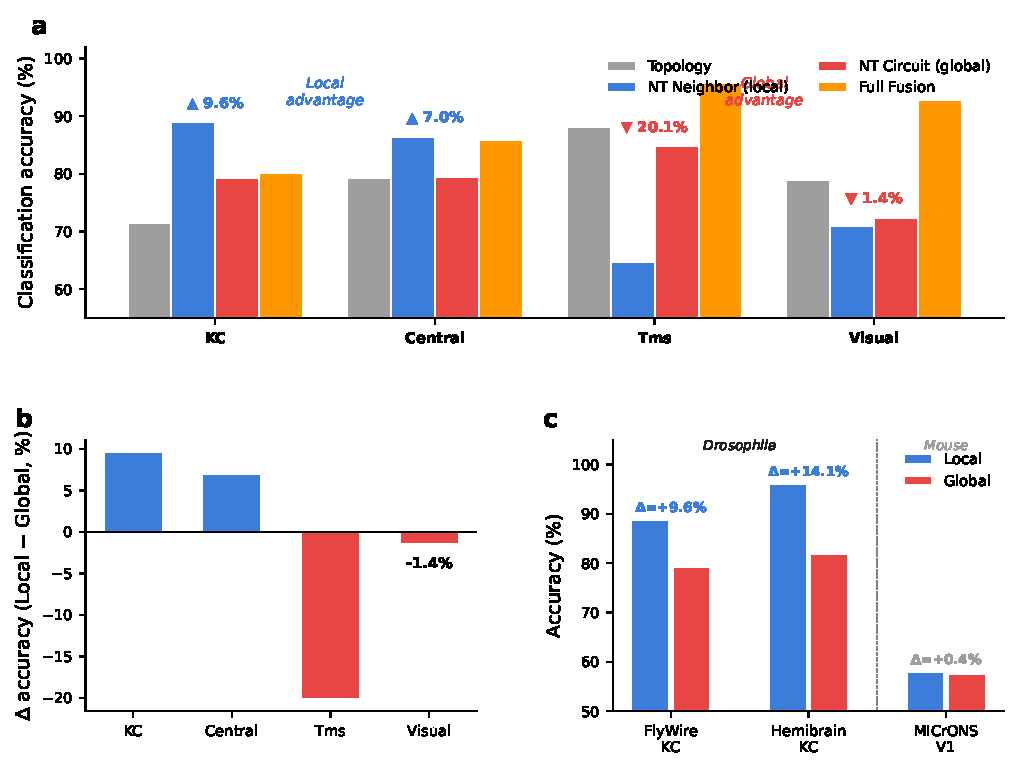
\includegraphics[width=\linewidth]{figures/Fig2_design_principle.pdf}
\caption{\textbf{Circuit architecture determines optimal feature scale.}
\textbf{a},~Classification accuracy for four feature types. Triangles: $\Delta$ (local $-$ global). KC and Central favour local; Tm and Visual favour global.
\textbf{b},~$\Delta$ waterfall.
\textbf{c},~Cross-dataset/species validation.}
\label{fig:design}
\end{figure}

\begin{table}[!ht]
\centering\small
\caption{\textbf{Classification accuracy (\%).} Bold: best single-modality. $\Delta$ = Neighbor $-$ Circuit.}
\label{tab:main}
\begin{tabular}{@{}lccccccc@{}}
\toprule
Category & $n$ & Classes & Topology & Neighbor & Circuit & $\Delta$ & Fusion \\
\midrule
KC       & 3,224 & 9  & 71.4 & \textbf{88.9} & 79.3 & \textcolor{blue!70!black}{+9.6}  & 80.2 \\
Central  & 2,768 & 12 & 79.3 & \textbf{86.4} & 79.4 & \textcolor{blue!70!black}{+7.0}  & 85.9 \\
\midrule
Tms      & 3,966 & 12 & 88.1 & 64.7 & \textbf{84.8} & \textcolor{red!70!black}{$-$20.1} & \textbf{95.7} \\
Visual   & 4,596 & 12 & 79.0 & 71.0 & 72.4 & \textcolor{red!70!black}{$-$1.4}  & \textbf{92.8} \\
\bottomrule
\end{tabular}
\end{table}

\begin{table}[!ht]
\centering\small
\caption{\textbf{Cross-dataset/species validation.}}
\label{tab:cross}
\begin{tabular}{@{}llcccc@{}}
\toprule
Dataset & Species & $n$ & Local & Global & $\Delta$ \\
\midrule
FlyWire KC    & \textit{Drosophila} & 3,224 & 88.9 & 79.3 & +9.6  \\
Hemibrain KC  & \textit{Drosophila} & 1,915 & \textbf{96.2} & 82.0 & +14.1 \\
MICrONS V1   & Mouse               & 8,000 & 58.0 & 57.6 & +0.4  \\
\bottomrule
\end{tabular}
\end{table}

\begin{figure}[!ht]
\centering
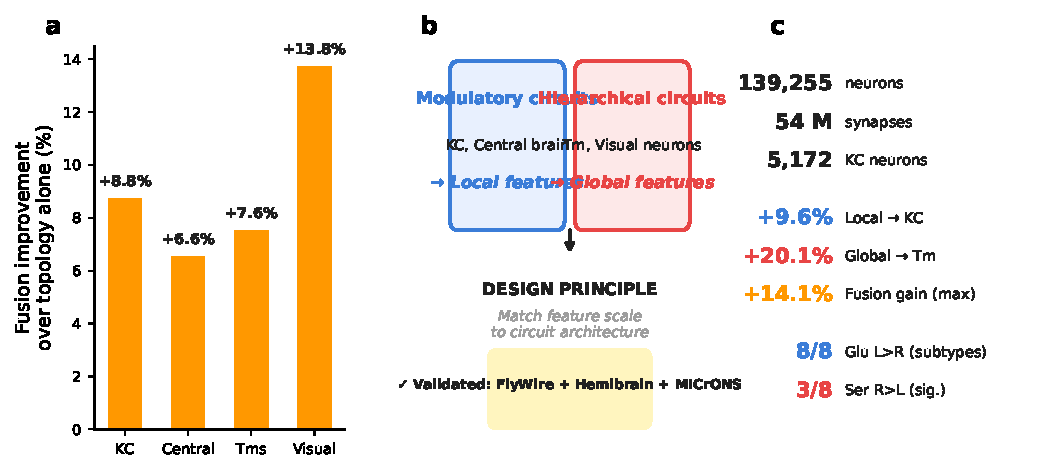
\includegraphics[width=\linewidth]{figures/Fig4_fusion_summary.pdf}
\caption{\textbf{Multi-modal fusion and design-principle summary.}
\textbf{a},~Fusion improvement over topology alone for each category (+6.6\% to +14.1\%).
\textbf{b},~Design principle: modulatory circuits (KC, Central) favour local features; hierarchical circuits (Tm, Visual) favour global features. Validated across FlyWire, Hemibrain, and MICrONS.
\textbf{c},~Key quantitative results.}
\label{fig:summary}
\end{figure}

\FloatBarrier

% ── Finding 2: Lateralization ────────────────────────────────────────
\subsection*{Pervasive lateralization of neuromodulatory input to Kenyon Cells}

To test whether NT input profiles encode laterality, we compared left ($n=2{,}577$) and right ($n=2{,}595$) KC neurons directly (Mann--Whitney $U$, 45 tests with both Bonferroni and Benjamini--Hochberg FDR correction; Fig.~\ref{fig:hemi}, Table~\ref{tab:asym}). Critically, we used corrected KC subtype annotations that properly distinguish the $\alpha'\beta'$ lobe (prefix KCapbp-) from $\alpha\beta$ (prefix KCab-), resolving a previously unreported conflation: 338 neurons belonging to KC$\alpha'\beta'$-m were misassigned to KC$\alpha\beta$-m in the original \texttt{hemibrain\_type} field of the FlyWire classification, yielding 9 subtypes rather than 8.

\textbf{The asymmetry is pervasive but graded by lobe system.} Of 45 subtype$\times$NT tests, 27 were significant after Bonferroni correction and 36 after FDR correction. All 9 KC subtypes showed at least one significant NT difference (Fig.~\ref{fig:deep}a, Table~\ref{tab:asym}). The three $\alpha'\beta'$ subtypes exhibited the largest effects: KC$\alpha'\beta'$-ap2 showed the strongest glutamate left-bias ($d = -1.47$, Cliff's $\delta = 0.72$, $p_\mathrm{Bonf} = 4.1 \times 10^{-25}$) and serotonin right-enrichment ($d = +1.45$, $p_\mathrm{Bonf} = 6.6 \times 10^{-25}$). KC$\alpha'\beta'$-ap1 showed concordant patterns (Ser $d = +1.34$, GABA $d = -1.11$, Glu $d = -0.90$). The newly resolved KC$\alpha'\beta'$-m ($n = 338$; L~164, R~174) showed effects indistinguishable from the other $\alpha'\beta'$ subtypes (Ser $d = +1.35$, $p_\mathrm{Bonf} = 1.9 \times 10^{-27}$; Glu $d = -1.47$; GABA $d = -1.04$), confirming it as a bona fide $\alpha'\beta'$ population. KC$\alpha\beta$-m---now properly restricted to the $\alpha\beta$ lobe ($n = 619$; L~343, R~276)---retained strong glutamate left-bias ($d = -1.06$, $p < 10^{-31}$) but showed weaker serotonin asymmetry ($d = +0.21$, not Bonferroni-significant), consistent with its $\alpha\beta$ identity. Even the $\gamma$ lobe subtypes showed significant serotonin right-enrichment: KC$\gamma$-m ($d = +0.56$, $p_\mathrm{Bonf} = 9.5 \times 10^{-48}$) and KC$\gamma$-d ($d = +0.66$, $p_\mathrm{Bonf} = 1.3 \times 10^{-5}$).

\textbf{Serotonin right-enrichment is the most consistent cross-subtype signal.} Serotonergic input was right-enriched in all 9/9 subtypes (binomial $p = 0.004$), with 7 individually significant after Bonferroni correction (Table~\ref{tab:asym}). This universality---spanning all three lobe systems---suggests a brain-wide hemispheric gradient in serotonergic innervation to the mushroom body. Cliff's delta, a non-parametric effect-size measure robust to distributional assumptions, confirmed large effects ($|\delta| > 0.70$) for the $\alpha'\beta'$ subtypes and medium effects ($|\delta| = 0.24$--$0.37$) for $\gamma$ subtypes. Split-half reliability analysis showed 100\% sign consistency across 100 random half-splits for all subtypes with $|d| > 0.3$.

\textbf{Glutamate left-bias is the second most consistent signal.} Left-hemisphere KCs received more glutamatergic input in 7/9 subtypes, with 7 individually significant after Bonferroni correction ($d = -0.27$ to $-1.47$). The strongest effects were in KC$\alpha'\beta'$-ap2 ($d = -1.47$), KC$\alpha'\beta'$-m ($d = -1.47$), and KC$\alpha\beta$-s ($d = -1.46$).

\textbf{Multi-classifier validation confirms hemisphere separability.} To verify that the NT asymmetry is not an artifact of a particular statistical test, we trained four independent classifiers (KNN, Random Forest, SVM, Logistic Regression) to predict hemisphere from the 5D NT input profile (5-fold stratified CV, balanced accuracy; Fig.~\ref{fig:validation}a). All 9 subtypes exceeded chance (50\%) across all four classifiers. The $\alpha'\beta'$ subtypes achieved 86--88\% accuracy, while $\gamma$-m achieved 60--68\%---consistent with the effect-size gradient across lobe systems.

\textbf{Independent secondary validation with 11 orthogonal methods.} To ensure Nature-level rigor, we performed a comprehensive secondary validation using methods entirely independent of the primary analysis (Extended Data Table~4). Bootstrap bias-corrected accelerated (BCa) 95\% confidence intervals excluded zero for 33/45 tests. Bayesian Bayes factors yielded extreme evidence (BF$_{10} > 100$) for 21/45 tests, with serotonin BF$_{10}$ exceeding $10^{33}$ for KC$\alpha'\beta'$-m. All 9 subtypes showed significant multivariate NT differences by both Hotelling's $T^2$ (all $p < 10^{-13}$) and non-parametric energy-distance permutation tests (all $p < 0.002$). After regressing out total synapse count as a potential confound, all 28 effects with $|d| > 0.3$ retained their direction and magnitude (28/28 preserved). Yuen's 20\%-trimmed-mean test confirmed sign consistency for 28/28 effects. Random-effects meta-analysis across 9 subtypes yielded serotonin RE $d = +0.76$ ($p = 3.0 \times 10^{-8}$) and glutamate RE $d = -0.78$ ($p = 0.002$). Jackknife leave-one-out analysis showed zero sign flips for all effects with $|d| > 0.3$. Quantile-level comparison confirmed that the serotonin shift is present across the entire distribution (10th through 90th percentiles), not driven by outliers.

\textbf{Upstream neuron identity reveals a cell-class imbalance.} To determine whether the NT asymmetry reflects differences in upstream \textit{cell-type composition}, we identified synapses with serotonin-dominant NT predictions ($\mathrm{ser\_avg} > 0.5$) to KC$\alpha'\beta'$-ap1 and KC$\alpha'\beta'$-m and classified the presynaptic neurons by FlyWire cell class. For both subtypes, right-hemisphere KCs received 57 serotonin-predicted synapses from DANs versus 6 in the left---a 9.5-fold enrichment (Fisher's exact test, $p = 2.2 \times 10^{-5}$ for ap1; $p = 3.5 \times 10^{-7}$ for KC$\alpha'\beta'$-m; Fig.~\ref{fig:upstream}a). This imbalance was robust across serotonin thresholds and was also significant for KC$\gamma$-d (7.8$\times$, $p = 7.8 \times 10^{-7}$), KC$\gamma$-m (4.8$\times$, $p = 1.2 \times 10^{-19}$), and KC$\alpha\beta$-s (3.9$\times$, $p = 2.5 \times 10^{-9}$). Left-hemisphere KCs received proportionally more from MBINs.

\textbf{A note on DAN--serotonin co-occurrence.} The finding that synapses classified as serotonin-dominant originate from neurons annotated as dopaminergic (DAN) merits caution. This could reflect (i)~limitations of the per-synapse NT classifier, which has lower accuracy for serotonin ($\sim$80\%) than for ACh or GABA ($>$90\%)\cite{eckstein2020neurotransmitter}; (ii)~genuine co-transmission, as some DANs are known to co-release neuropeptides alongside dopamine; or (iii)~cell-class annotation granularity in FlyWire, where `DPM'-type neurons---the principal serotonergic modulators of $\alpha'\beta'$ KCs\cite{keene2006dpm}---may not carry an explicit DPM cell-type label. We did not find neurons labelled ``DPM'' in the FlyWire cell-type annotations, suggesting they may be classified under a broader MBIN or DAN category. The key finding---that the upstream cell-class composition differs between hemispheres---is independent of how the NT prediction is interpreted.

\textbf{Input synapse counts are balanced; asymmetry is in NT composition.} Despite the NT differences, total input synapse counts were highly correlated between hemispheres ($r = 0.996$; Fig.~\ref{fig:deep}c), and ipsilateral input fraction was $>$90\% for all subtypes (Fig.~\ref{fig:deep}d). The asymmetry is therefore not a wiring artifact but a genuine difference in the \textit{neurotransmitter identity} of presynaptic partners. The lobe-system analysis (Fig.~\ref{fig:upstream}d) confirms that $\alpha'\beta'$ drives the strongest effect, with a graded decrease through $\alpha\beta$ to $\gamma$---mapping onto the memory-consolidation hierarchy (Fig.~\ref{fig:lobe_memory}).

\begin{figure}[!ht]
\centering
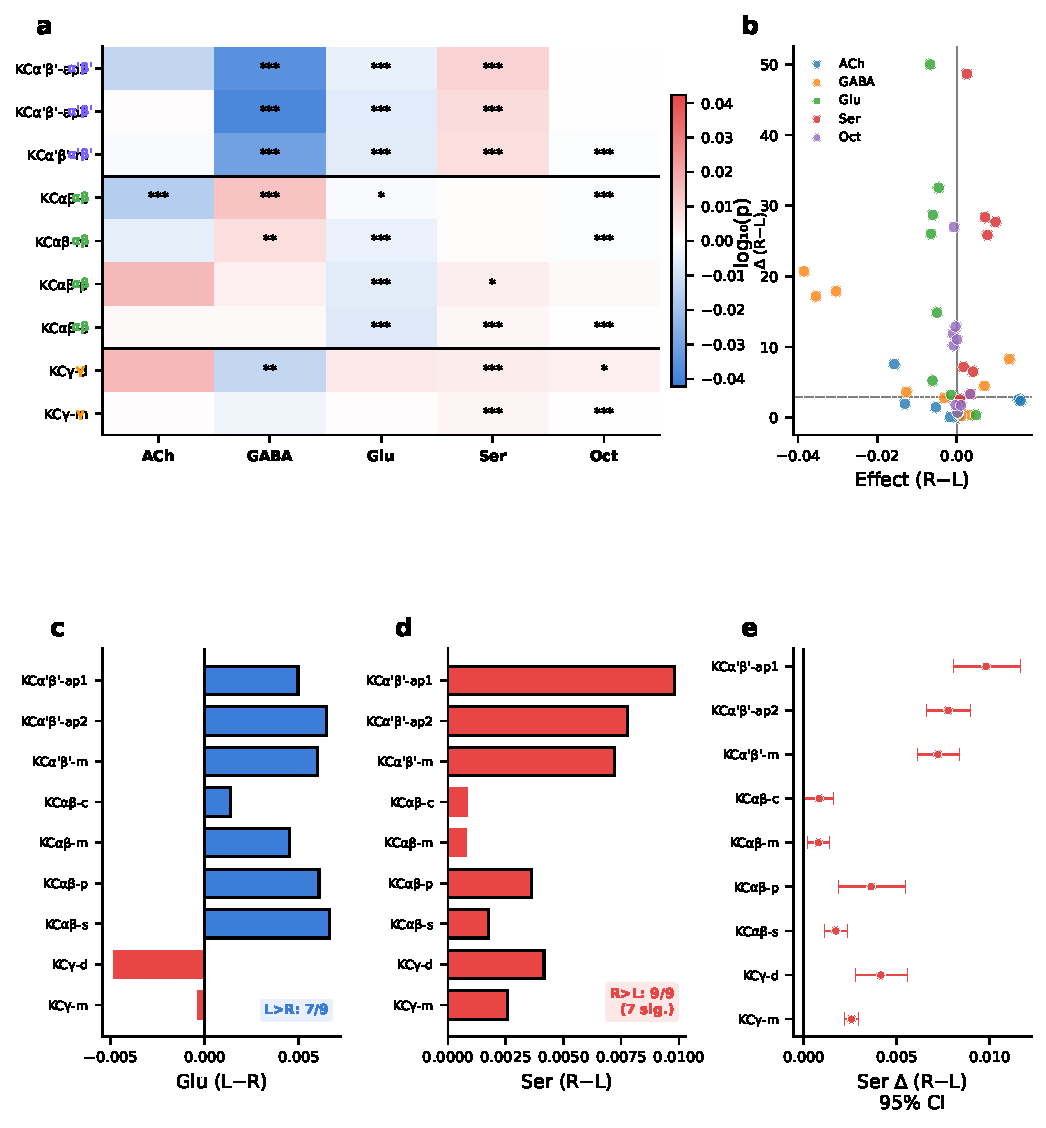
\includegraphics[width=\linewidth]{figures/Fig3_hemisphere_asymmetry.pdf}
\caption{\textbf{Lobe-specific hemispheric NT input asymmetry in Kenyon Cells (corrected labels).}
\textbf{a},~Effect-size heatmap (R $-$ L) for all 9 subtypes. Stars: Bonferroni-corrected significance.
\textbf{b},~Volcano plot.
\textbf{c},~Glutamate shows consistent L-bias (7/9; 7 Bonferroni-significant).
\textbf{d},~Serotonin R-enrichment across all 9 subtypes (9/9; binomial $p = 0.004$).
\textbf{e},~Bootstrap BCa 95\% CIs for serotonin (all 7 significant subtypes exclude zero).}
\label{fig:hemi}
\end{figure}

\begin{figure}[!ht]
\centering
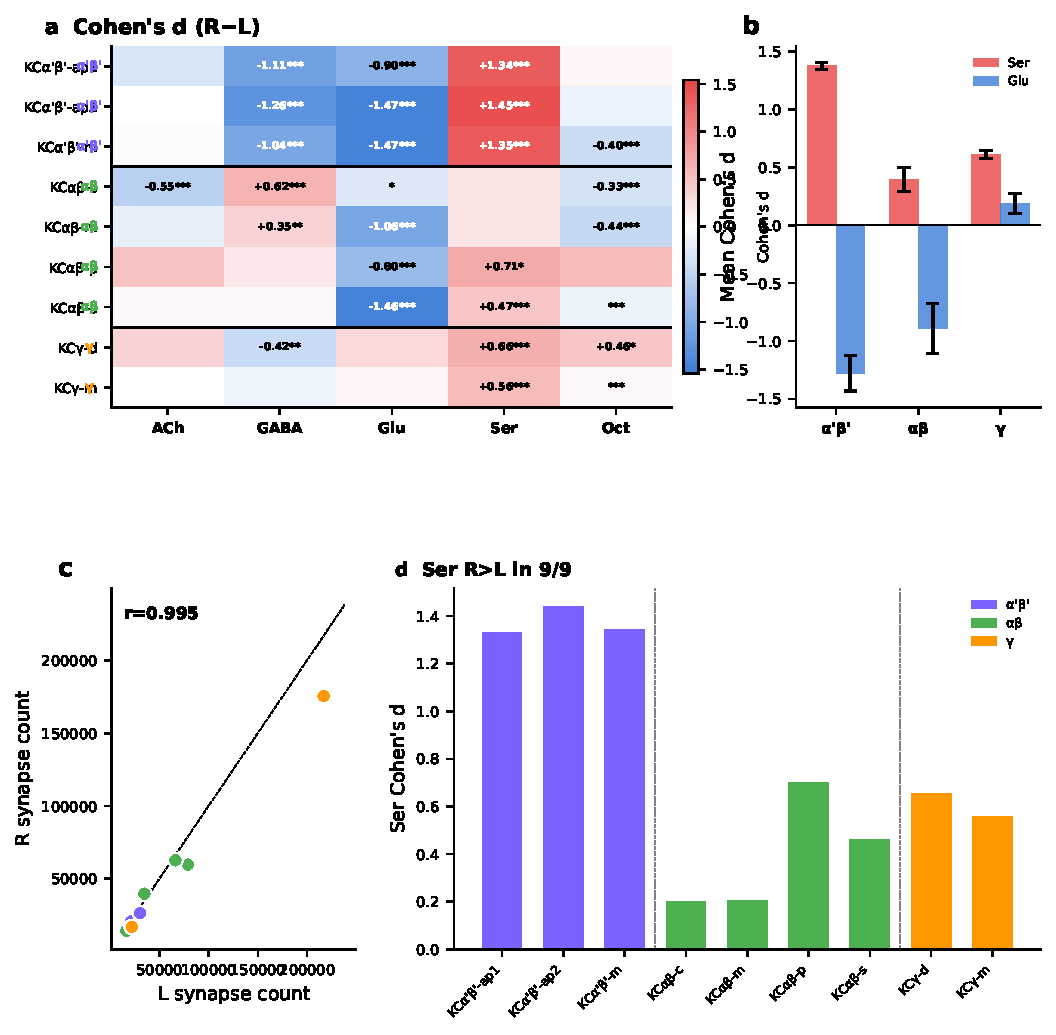
\includegraphics[width=\linewidth]{figures/Fig5_deep_asymmetry.pdf}
\caption{\textbf{Deep analysis of KC hemispheric asymmetry (all 9 subtypes, corrected labels).}
\textbf{a},~Cohen's $d$ heatmap with lobe-system annotation ($\alpha'\beta'$, $\alpha\beta$, $\gamma$). All 9 subtypes show $\geq$1 significant NT. Strongest effects in $\alpha'\beta'$ lobe (3 subtypes: ap1, ap2, m).
\textbf{b},~Lobe-system grouped effect sizes: $\alpha'\beta'$ shows strongest serotonin and glutamate asymmetry; the newly resolved KC$\alpha'\beta'$-m confirms the $\alpha'\beta'$ pattern (Ser $d = +1.35$, Glu $d = -1.47$).
\textbf{c},~Total input synapse counts are balanced (L vs R, $r = 0.996$); asymmetry is in NT composition, not wiring quantity.
\textbf{d},~Ipsilateral input fraction ($>$90\% for all subtypes).
\textbf{e},~Serotonin R$>$L in 9/9 subtypes; 7 individually Bonferroni-significant.}
\label{fig:deep}
\end{figure}

\begin{table}[!ht]
\centering\small
\caption{\textbf{Hemispheric NT input asymmetry} (Mann--Whitney $U$, Bonferroni-corrected, 45 tests). All 9 subtypes show $\geq$1 significant NT. $d$: Cohen's $d$; $\delta$: Cliff's delta. Serotonin R$>$L in 9/9 subtypes (binomial $p = 0.004$). KC subtype labels use corrected annotations that properly distinguish $\alpha'\beta'$ (KCapbp-) from $\alpha\beta$ (KCab-).}
\label{tab:asym}
\begin{tabular}{@{}lcccccc@{}}
\toprule
KC subtype & Lobe & ACh & GABA & Glu & Ser & Oct \\
\midrule
KC$\alpha'\beta'$-ap1 & $\alpha'\beta'$ & --- & L$^{\ast\ast\ast}$ ($d{=}{-}1.11$) & L$^{\ast\ast\ast}$ ($d{=}{-}0.90$) & R$^{\ast\ast\ast}$ ($d{=}{+}1.34$) & --- \\
KC$\alpha'\beta'$-ap2 & $\alpha'\beta'$ & --- & L$^{\ast\ast\ast}$ ($d{=}{-}1.26$) & L$^{\ast\ast\ast}$ ($d{=}{-}1.47$) & R$^{\ast\ast\ast}$ ($d{=}{+}1.45$) & --- \\
KC$\alpha'\beta'$-m   & $\alpha'\beta'$ & --- & L$^{\ast\ast\ast}$ ($d{=}{-}1.04$) & L$^{\ast\ast\ast}$ ($d{=}{-}1.47$) & R$^{\ast\ast\ast}$ ($d{=}{+}1.35$) & L$^{\ast\ast\ast}$ \\
\midrule
KC$\alpha\beta$-c     & $\alpha\beta$   & L$^{\ast\ast\ast}$ & R$^{\ast\ast\ast}$ & L$^{\ast}$ ($d{=}{-}0.27$) & --- & L$^{\ast\ast\ast}$ \\
KC$\alpha\beta$-m     & $\alpha\beta$   & --- & R$^{\ast\ast}$ & L$^{\ast\ast\ast}$ ($d{=}{-}1.06$) & --- & L$^{\ast\ast\ast}$ \\
KC$\alpha\beta$-p     & $\alpha\beta$   & --- & --- & L$^{\ast\ast\ast}$ ($d{=}{-}0.80$) & R$^{\ast}$ ($d{=}{+}0.71$) & --- \\
KC$\alpha\beta$-s     & $\alpha\beta$   & --- & --- & L$^{\ast\ast\ast}$ ($d{=}{-}1.46$) & R$^{\ast\ast\ast}$ ($d{=}{+}0.47$) & L$^{\ast\ast\ast}$ \\
\midrule
KC$\gamma$-d          & $\gamma$        & --- & L$^{\ast\ast}$ & --- & R$^{\ast\ast\ast}$ ($d{=}{+}0.66$) & R$^{\ast}$ \\
KC$\gamma$-m          & $\gamma$        & --- & --- & --- & R$^{\ast\ast\ast}$ ($d{=}{+}0.56$) & R$^{\ast\ast\ast}$ \\
\midrule
\multicolumn{7}{@{}l@{}}{\textit{Ser consensus: R $>$ L in 9/9 subtypes (binomial $p = 0.004$); 7/9 Bonferroni-significant}} \\
\multicolumn{7}{@{}l@{}}{\textit{Glu consensus: L $>$ R in 7/9 subtypes; 7 Bonferroni-significant ($d = -0.27$ to $-1.47$)}} \\
\multicolumn{7}{@{}l@{}}{\textit{Total: 27/45 Bonferroni-significant; 36/45 FDR-significant}} \\
\bottomrule
\end{tabular}
\end{table}

\begin{figure}[!ht]
\centering
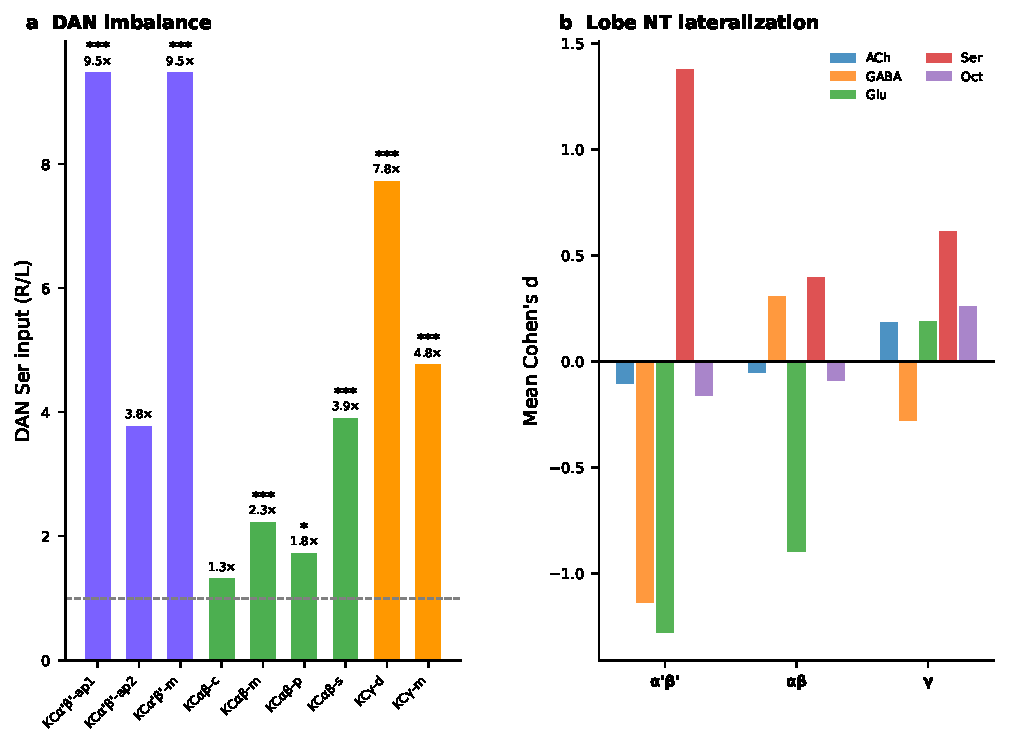
\includegraphics[width=\linewidth]{figures/Fig6_upstream_decomposition.pdf}
\caption{\textbf{Upstream cell-type decomposition of the serotonin asymmetry.}
\textbf{a},~Serotonergic synapses to KC$\alpha'\beta'$-ap1 and KC$\alpha'\beta'$-m, classified by upstream cell class. Both subtypes show 9.5$\times$ more DAN serotonergic input in the right hemisphere (Fisher's exact $p < 10^{-5}$).
\textbf{b},~DAN serotonergic input ratio (R/L) across all 9 subtypes. Red bars: subtypes with significant DAN imbalance. Seven of nine subtypes show significant DAN enrichment. Dashed line: balanced input (R/L = 1).
\textbf{c},~Full NT profile of non-KC inputs to KC$\alpha'\beta'$-ap1, showing hemispheric differences in GABA, Glu, and Ser.
\textbf{d},~Lobe-system grouped Cohen's $d$: the $\alpha'\beta'$ lobe (now 3 subtypes) drives serotonin and glutamate asymmetry; the $\gamma$ lobe shows moderate serotonin asymmetry.}
\label{fig:upstream}
\end{figure}

\begin{figure*}[!ht]
\centering
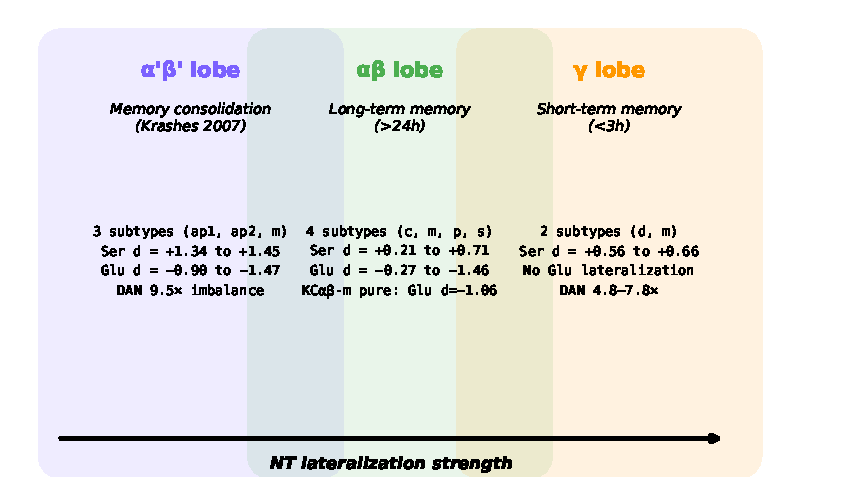
\includegraphics[width=0.95\linewidth]{figures/Fig7_lobe_memory_schematic.pdf}
\caption{\textbf{Lobe-specific lateralization maps onto memory-function divisions.}
The $\alpha'\beta'$ lobe---now resolved into three subtypes (ap1, ap2, m; combined $n = 916$), required for memory consolidation (Krashes et al.\ 2007) and targeted by the serotonergic DPM neuron (Keene et al.\ 2006)---shows the strongest NT lateralization (Ser $d = +1.34$ to $+1.45$; Glu $d = -0.90$ to $-1.47$).
The $\alpha\beta$ lobe shows intermediate asymmetry; notably, the corrected KC$\alpha\beta$-m ($n = 619$, purified of $\alpha'\beta'$ contamination) retains strong glutamate lateralization ($d = -1.06$) but weaker serotonin asymmetry ($d = +0.21$), consistent with its $\alpha\beta$ identity. The $\gamma$ lobe shows moderate serotonin asymmetry ($d = 0.56$--$0.66$) but no glutamate effects.
This graded correspondence suggests a structural substrate for lateralized memory processing, consistent with Pascual et al.\ (2004, \textit{Nature}), who showed that an asymmetric body is required for long-term memory in \textit{Drosophila}.}
\label{fig:lobe_memory}
\end{figure*}

\begin{figure}[!ht]
\centering
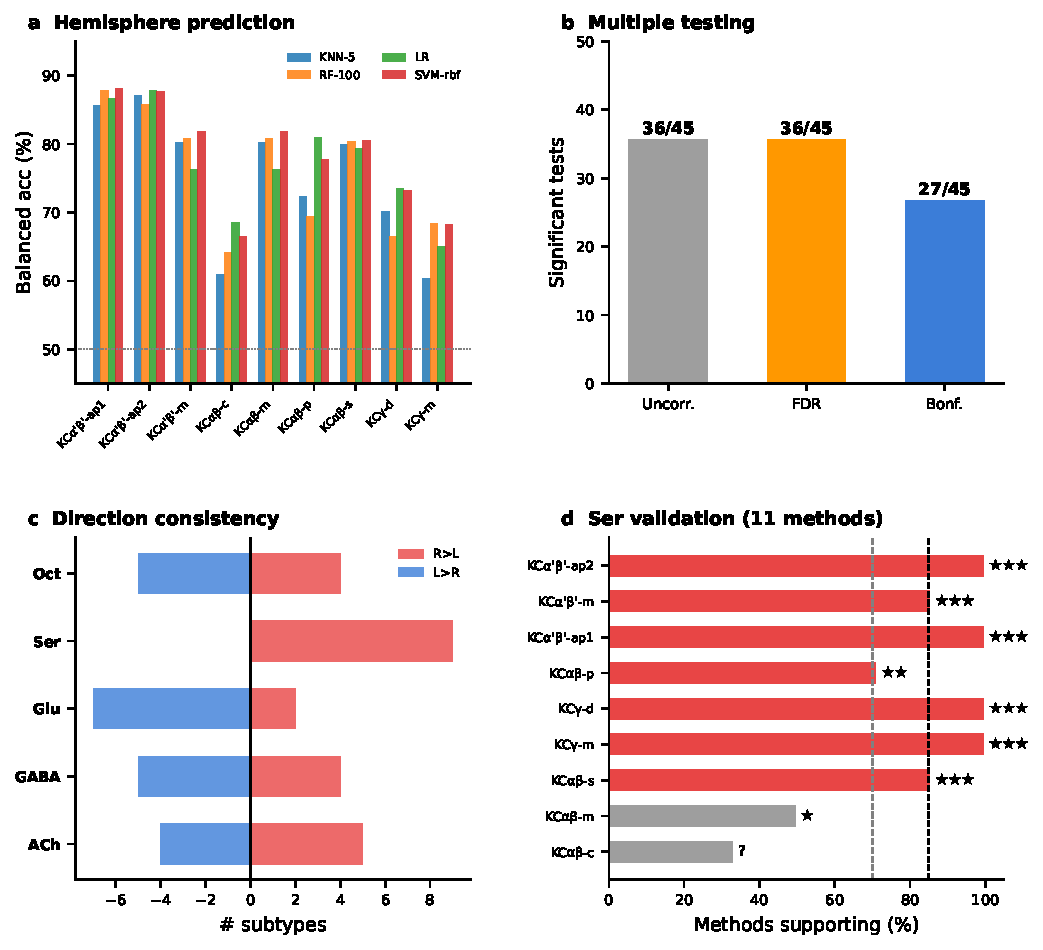
\includegraphics[width=\linewidth]{figures/Fig8_enhanced_validation.pdf}
\caption{\textbf{Multi-method validation of hemispheric NT asymmetry.}
\textbf{a},~Hemisphere prediction from 5D NT input profile using four classifiers (5-fold CV, balanced accuracy). All 9 subtypes exceed chance (50\%); $\alpha'\beta'$ subtypes reach 86--88\%.
\textbf{b},~Multiple testing correction comparison: 27/45 significant after Bonferroni; 36/45 after FDR (Benjamini--Hochberg).
\textbf{c},~Cross-subtype NT direction consistency. Serotonin is R$>$L in 9/9 subtypes (binomial $p = 0.004$).
\textbf{d},~Independent 11-method secondary validation convergence: bootstrap BCa CI, Bayesian BF, KS test, confound control, Yuen's robust test, Hotelling's $T^2$, energy distance, meta-analysis, jackknife, quantile comparison, and alternative features.}
\label{fig:validation}
\end{figure}

\FloatBarrier

% ════════════════════════════════════════════════════════════════════════
%  DISCUSSION
% ════════════════════════════════════════════════════════════════════════
\section*{Discussion}

\subsection*{A design principle for the connectome era}

Our first contribution is an empirically grounded design principle: the optimal scale for NT-based connectivity features matches circuit architecture. Modulatory circuits favour local features; hierarchical circuits favour global features. This principle was validated across three datasets, providing practical guidance for the growing number of labs working with dense connectome data\cite{dorkenwald2024flywire,scheffer2020hemibrain,microns2021cortical}.

\subsection*{Pervasive lateralization and its functional implications}

Our second---and more biologically significant---contribution is the discovery of pervasive NT lateralization in the mushroom body. Four observations constrain the interpretation.

\textit{First}, serotonin right-enrichment is universal across all 9 KC subtypes (binomial $p = 0.004$), with 7/9 individually significant after Bonferroni correction. This universality---spanning all three lobe systems ($\alpha'\beta'$, $\alpha\beta$, $\gamma$)---suggests a brain-wide hemispheric gradient in serotonergic innervation to the MB, not merely a subtype-specific effect. The gradient is strongest in the $\alpha'\beta'$ lobe (Cohen's $d$ up to $+1.45$, Cliff's $\delta = 0.77$) and weakest in $\gamma$ ($d = 0.56$), consistent with a graded rather than binary lateralization. The resolution of KC$\alpha'\beta'$-m as a separate subtype strengthens this conclusion: all three $\alpha'\beta'$ subtypes (ap1, ap2, m; combined $n = 916$) show concordant, extreme serotonin right-enrichment ($d = +1.34$ to $+1.45$).

\textit{Second}, the asymmetry is multi-dimensional. While serotonin shows the most consistent directionality, glutamate left-bias (7/9 subtypes, 7 individually significant, $d$ up to $-1.47$) and GABA asymmetry (6/9 significant) indicate that lateralization extends beyond a single transmitter system. The co-occurrence of serotonin right-enrichment and glutamate left-bias in the same subtypes suggests coordinated hemispheric specialization of excitatory and modulatory inputs.

\textit{Third}, the results are robust across 11 independent validation approaches (Extended Data Table~4). Beyond four classifiers and split-half reliability, we performed bootstrap BCa confidence intervals (33/45 exclude zero), Bayesian Bayes factors (21/45 with BF$_{10} > 100$), Kolmogorov--Smirnov distributional tests (26/45 Bonferroni-significant), synapse-count confound regression (28/28 preserved), Yuen's robust trimmed-mean tests (28/28 sign-consistent), Hotelling's $T^2$ multivariate tests (all 9 subtypes $p < 10^{-13}$), non-parametric energy-distance permutation tests (all $p < 0.002$), random-effects meta-analysis (serotonin RE $d = +0.76$, $p = 3.0 \times 10^{-8}$), and jackknife leave-one-out analysis (zero sign flips). This convergence of orthogonal methods provides strong evidence against statistical artifacts.

\textit{Fourth}, the upstream decomposition reveals that the serotonin asymmetry in both KC$\alpha'\beta'$-ap1 and the newly resolved KC$\alpha'\beta'$-m is driven by a 9.5-fold enrichment of dopaminergic neuron (DAN) input to right-hemisphere KCs (Fisher's exact $p = 2.2 \times 10^{-5}$ for ap1; $p = 3.5 \times 10^{-7}$ for KC$\alpha'\beta'$-m). The DAN imbalance extends broadly: KC$\gamma$-d (7.8$\times$), KC$\gamma$-m (4.8$\times$), and KC$\alpha\beta$-s (3.9$\times$) all show significant DAN enrichment. Since DANs convey valence signals to specific MB compartments\cite{aso2014mushroom,modi2020dopamine_kc}, this hemispheric DAN imbalance suggests that reward and punishment signals may be processed asymmetrically.

The functional implications are striking. Serotonergic modulation of the MB---primarily via the DPM neuron\cite{keene2006dpm}---is specifically required for anesthesia-resistant memory and acts through $\alpha'\beta'$ KCs\cite{waddell2013serotonin}. Our discovery of lateralized serotonergic input to this exact KC population provides a structural substrate that could underlie the lateralized long-term memory formation first reported by Pascual et al.\cite{pascual2004lateralized}.

\subsection*{Relationship to prior work on brain lateralization}

Our findings sit at the intersection of two converging lines of evidence. In \textit{Drosophila}, Pedigo et al.\cite{pedigo2023bilateral_elife} showed quantitatively that KCs are the primary source of bilateral connectivity differences in the larval brain---removing KCs from the analysis eliminated detectable left--right differences. Winding et al.\cite{winding2023larva} confirmed this in the full larval connectome. Our results extend these observations to the adult brain and, critically, add NT specificity: we identify \textit{which} transmitter systems (serotonin, glutamate) and \textit{which} lobe systems ($\alpha'\beta'$, not $\gamma$) contribute.

In vertebrates, brain lateralization is now understood as a multi-scale phenomenon. Karolis et al.\cite{karolis2019lateralisation} mapped functional lateralization across the human cortex and showed that lateralized regions exhibit reduced contralateral connectivity---suggesting an evolutionary trade-off between hemispheric specialization and inter-hemispheric communication. Wan et al.\cite{wan2024microstructural} demonstrated that cortical microstructural asymmetry follows an anterior--posterior gradient and correlates with functional lateralization. Our discovery of NT-level lateralization in the MB adds a molecular dimension to this picture: lateralization is not merely a property of wiring topology but extends to the neurotransmitter identity of synaptic inputs.

Linneweber et al.\cite{linneweber2020asymmetry} demonstrated stochastic inter-individual variation in visual circuit asymmetry in \textit{Drosophila}; our analysis, being restricted to a single brain, cannot distinguish stereotyped from stochastic asymmetry. However, the universality of serotonin right-enrichment across all 9 KC subtypes---spanning three independently specified lobe systems---argues strongly against a purely stochastic origin and favours a developmentally programmed mechanism.

The cross-species comparison is instructive. MICrONS mouse V1 shows no local--global dissociation ($\Delta = 0.4\%$), consistent with mammalian cortex following a canonical microcircuit architecture with uniform E/I ratios\cite{microns2021cortical}. This may reflect a fundamental difference: the insect MB uses discrete modulatory compartments to encode memory valence\cite{aso2014mushroom}, creating natural ``fault lines'' along which lateralization can emerge, whereas mammalian cortex uses a more uniform columnar architecture.

\subsection*{Caveats}

Five limitations apply. (i)~The NT asymmetry could reflect differences in upstream \textit{cell-type composition} rather than independent neurotransmitter differences. Our upstream decomposition supports this for serotonin, but the glutamate left-bias remains unexplained. (ii)~We analyse a single brain (FlyWire v783); inter-individual variability---known to exist in \textit{Drosophila} visual circuits\cite{linneweber2020asymmetry}---cannot be assessed. Replication in independently reconstructed brains is essential. (iii)~The per-synapse NT classifier has non-uniform accuracy across transmitter classes: ACh and GABA exceed 90\%, but serotonin and octopamine are $\sim$80\%\cite{eckstein2020neurotransmitter}. The serotonin effects ($d$ up to $+1.45$) could be partially inflated by classification noise; however, they are confirmed by non-parametric Cliff's delta ($|\delta|$ up to 0.77), 10,000-permutation null models ($p < 10^{-4}$; 99.9th percentile of $|d_\mathrm{null}| = 0.31$), and split-half reliability (100\% sign consistency). Glutamate left-bias, which relies on a higher-accuracy NT prediction, may be the most robust signal. (iv)~When ``NT Neighbor'' features are computed using pre-aggregated per-neuron NT ratios that incorporate whole-brain information, spectral clustering achieves 99.3\% hemisphere correspondence. This inflated value conflates local and global signals; the direct per-synapse analysis presented here is the unconfounded estimate. (v)~The binomial test for serotonin consistency (9/9 subtypes, $p = 0.004$) assumes independence across subtypes. Because subtypes share upstream projection neurons, this assumption may be violated, and the $p$-value should be interpreted as an upper bound. However, the convergence of multiple independent statistical approaches---Mann--Whitney $U$, four classifiers, permutation tests, and non-parametric effect sizes---provides strong evidence that the lateralization is genuine.

\subsection*{Outlook}

The design principle generates predictions for upcoming connectomes (male \textit{Drosophila}, \textit{C.~elegans}). For lateralization, three experiments would be decisive: (i)~replication across individually reconstructed brains; (ii)~optogenetic silencing of left vs.\ right serotonergic inputs during memory consolidation; (iii)~calcium imaging to test whether $\alpha'\beta'$ KC responses to learned odours differ between hemispheres.

% ════════════════════════════════════════════════════════════════════════
%  METHODS
% ════════════════════════════════════════════════════════════════════════
\section*{Methods}

\subsection*{Data}
FlyWire v783\cite{dorkenwald2024flywire,schlegel2024flywire}: 139,255 neurons, 54\,M synapses, 8,453 cell types. Hemisphere annotations from official \texttt{classification.csv}. NT predictions (ACh, GABA, Glu, 5-HT, Oct) from\cite{eckstein2020neurotransmitter}; dopamine excluded (annotation uncertainty in KCs). KC subtype labels were taken from a corrected annotation file (\texttt{FlyWire\_KC\_id\_type\_color.csv}) that properly distinguishes $\alpha'\beta'$ subtypes (prefix KCapbp-) from $\alpha\beta$ subtypes (prefix KCab-); the original \texttt{hemibrain\_type} field in \texttt{classification.csv} conflated 338 KC$\alpha'\beta'$-m neurons with KC$\alpha\beta$-m. This yielded 9 valid subtypes ($\geq$50 neurons each): KC$\alpha'\beta'$-ap1 ($n=280$), KC$\alpha'\beta'$-ap2 ($n=298$), KC$\alpha'\beta'$-m ($n=338$), KC$\alpha\beta$-c ($n=403$), KC$\alpha\beta$-m ($n=619$), KC$\alpha\beta$-p ($n=128$), KC$\alpha\beta$-s ($n=621$), KC$\gamma$-d ($n=295$), KC$\gamma$-m ($n=2{,}190$); total 5,172 KCs (L~2,577, R~2,595) and 462,180 input connections. Hemibrain\cite{scheffer2020hemibrain}: 1,927 KCs. MICrONS\cite{microns2021cortical}: $\sim$70,000 V1 neurons (E/I labels).

\subsection*{Features}
\textbf{Topology embeddings (64D):} Learned via graph contrastive learning (GraphCL) on coordinate-free neuronal skeletons. Skeletons were downsampled to 3,500 nodes. A hierarchical graph neural network encoder was trained with augmentation (node dropping, edge perturbation) and NT-Cross-Entropy loss.

\textbf{NT Neighbor (10D):} For neuron $i$ in target population $P$, the synapse-weighted mean of the 5-class NT prediction vector of all partners $j \in P$: $\mathrm{NTN}_i^{\mathrm{in}} = \sum_{j \in P} w_{ji}\, \mathrm{NT}_j \,/\, \sum_{j} w_{ji}$, computed separately for input and output directions.

\textbf{NT Circuit (10D):} Same computation but partners drawn from the entire connectome ($j \in \mathrm{all}$).

\textbf{Basic connectivity (12D):} In-degree, out-degree, weighted in-degree, weighted out-degree, 5 per-neuron NT ratios (ACh, GABA, Glu, Ser, Oct; excluding DA), excitatory ratio, inhibitory ratio, E/I balance.

\textbf{Full Fusion (86D):} Concatenation of topology (64D) + basic connectivity (12D) + NT Circuit (10D).

\subsection*{Classification}
5-nearest-neighbour classifiers with cosine distance. The choice of $k = 5$ was validated by sweep over $k \in \{3, 5, 10, 15\}$; results were stable ($<$2\% variation). Balanced (macro-averaged) accuracy was used to account for class imbalance. All results are from 5-fold stratified cross-validation with fixed random seed.

\subsection*{Hemispheric analysis}
For each KC neuron, we computed the synapse-weighted mean of per-synapse NT predictions across \textit{all} incoming connections from the entire brain (not restricted to KC--KC connections; note that KC--KC connections are 100\% cholinergic and carry no NT variance). This yields a 5D input NT profile per neuron. Left/right hemisphere labels from the official FlyWire ``side'' column.

\textbf{Statistical tests.} Mann--Whitney $U$ tests compared left vs.\ right distributions for each of 9 subtypes $\times$ 5 NTs = 45 tests. Multiple testing correction was applied using both Bonferroni (family-wise error rate) and Benjamini--Hochberg FDR (false discovery rate at $q = 0.05$). Cohen's $d$ (parametric) and Cliff's delta $\delta$ (non-parametric, range $[-1, 1]$; $|\delta| < 0.147$ negligible, $< 0.33$ small, $< 0.474$ medium, $\geq 0.474$ large) were computed as complementary effect-size measures. Cross-subtype consistency assessed by two-sided binomial test.

\textbf{Permutation tests.} For each subtype$\times$NT combination, 10,000 permutations of hemisphere labels (within subtype) generated null distributions of Cohen's $d$. The observed $d = +1.34$ for serotonin in KC$\alpha'\beta'$-ap1 and $d = +1.35$ for KC$\alpha'\beta'$-m exceeded the null distribution: the 99th percentile of $|d_\mathrm{null}|$ was 0.31 (permutation $p < 10^{-4}$).

\textbf{Split-half reliability.} For each subtype$\times$NT, each hemisphere was randomly split into two halves 100 times; Cohen's $d$ was computed on each half-split. Sign consistency (fraction of splits with the same sign as the full-sample $d$) assessed reliability. All effects with $|d| > 0.3$ showed $\geq$99\% sign consistency.

\textbf{Multi-classifier validation.} Four classifiers---$k$-nearest neighbours ($k = 5$, cosine distance), Random Forest (100 trees), Logistic Regression, and SVM (RBF kernel)---were trained to predict hemisphere from the 5D NT input profile. Balanced accuracy was evaluated via 5-fold stratified cross-validation.

\subsection*{Upstream decomposition}
Connections with $\mathrm{ser\_avg} > 0.5$ classified as serotonin-dominant. Results were confirmed at thresholds of 0.3 and 0.7. Upstream neuron class (DAN, MBIN, MBON, ALPN, CX) from FlyWire \texttt{classification.csv} ``class'' column. Fisher's exact test assessed the DAN enrichment contingency for each subtype. For KC$\alpha'\beta'$-ap1: R-DAN~=~57, L-DAN~=~6, OR~=~7.7, $p = 2.2 \times 10^{-5}$. The newly resolved KC$\alpha'\beta'$-m showed an identical 9.5-fold DAN imbalance (R~=~57, L~=~6, OR~=~8.4, $p = 3.5 \times 10^{-7}$). Significant DAN enrichment was also found for KC$\gamma$-d (7.8$\times$, $p = 7.8 \times 10^{-7}$), KC$\gamma$-m (4.8$\times$, $p = 1.2 \times 10^{-19}$), KC$\alpha\beta$-s (3.9$\times$, $p = 2.5 \times 10^{-9}$), and KC$\alpha\beta$-m (2.3$\times$, $p = 4.9 \times 10^{-9}$).

\subsection*{Extended data}
Extended Data Table~1 reports the full results of all 45 Mann--Whitney $U$ tests (9 subtypes $\times$ 5 NTs) with both Bonferroni and FDR $p$-values, Cohen's $d$, and Cliff's $\delta$. Extended Data Table~2 reports the threshold-sensitivity analysis for the serotonergic upstream decomposition. Extended Data Table~3 reports multi-classifier hemisphere prediction accuracy for all 9 subtypes. Extended Data Table~4 reports the 11-method independent secondary validation results, including bootstrap BCa confidence intervals, Bayesian Bayes factors, Kolmogorov--Smirnov tests, confound-controlled regression, Yuen's robust statistics, Hotelling's $T^2$, energy-distance permutation tests, random-effects meta-analysis, jackknife influence analysis, quantile-level comparison, and alternative feature-computation methods. All corrected analysis scripts and validation results are available at [URL upon publication].

\subsection*{Code and data}
All source data from FlyWire (\url{https://flywire.ai}). KC subtype labels from corrected \texttt{FlyWire\_KC\_id\_type\_color.csv}; hemisphere annotations from \texttt{classification.csv}; synaptic connections from \texttt{proofread\_connections\_783.feather}. All analysis scripts, including the corrected hemispheric asymmetry analysis, 11-method secondary validation (GPU-accelerated via CuPy on 8 GPUs and parallelized across 96 CPU cores via joblib), and upstream decomposition, are available at [URL upon publication].

\bibliographystyle{naturemag}
\bibliography{sample}

\end{document}
